
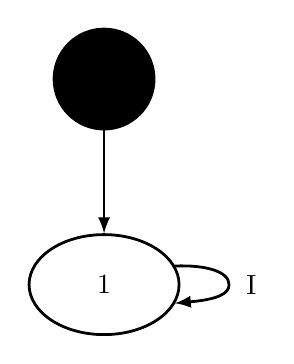
\begin{tikzpicture}[>=latex,line join=bevel,]
  \pgfsetlinewidth{1bp}
%%
\pgfsetcolor{black}
  % Edge: 0 -> 1
  \draw [->] (27.0bp,73.937bp) .. controls (27.0bp,65.807bp) and (27.0bp,55.876bp)  .. (27.0bp,36.441bp);
  % Edge: 1 -> 1
  \draw [->] (52.443bp,24.691bp) .. controls (63.028bp,25.152bp) and (72.0bp,22.922bp)  .. (72.0bp,18.0bp) .. controls (72.0bp,14.77bp) and (68.136bp,12.699bp)  .. (52.443bp,11.309bp);
  \definecolor{strokecol}{rgb}{0.0,0.0,0.0};
  \pgfsetstrokecolor{strokecol}
  \draw (80.0bp,18.0bp) node {I};
  % Node: 1
\begin{scope}
  \definecolor{strokecol}{rgb}{0.0,0.0,0.0};
  \pgfsetstrokecolor{strokecol}
  \draw (27.0bp,18.0bp) ellipse (27.0bp and 18.0bp);
  \draw (27.0bp,18.0bp) node {1};
\end{scope}
  % Node: 0
\begin{scope}
  \definecolor{strokecol}{rgb}{0.0,0.0,0.0};
  \pgfsetstrokecolor{strokecol}
  \definecolor{fillcol}{rgb}{0.0,0.0,0.0};
  \pgfsetfillcolor{fillcol}
  \filldraw [opacity=1] (27.0bp,92.0bp) ellipse (18.0bp and 18.0bp);
\end{scope}
%
\end{tikzpicture}

